\section{Auxiliary tables and figures for US, UK, and France}\label{app:US}\setcounter{equation}{0}
\subsection{Calibration}
For the US, we use the CPS March Supplement 2019 to identify low, medium, and high income cohorts. Income groups are designed to ensure that the "low" and "medium" income groups represent half-mean and mean income. This is used to identify the $\theta$ from the relative replacement rates reported in the OECD report Pensions at a Glance \parencite{OECDpen}. For the propensity to vote, we use US Census data for 2020 on Voting and Registration in the Election of November 2020. For the US pension spending, we use the OECD report Pensions at a Glance \parencite{OECDpen} and include Medicare spending from the the Medicare Payment Advisory Commission 2020 Data Book. 

%% GENERATED by python/paper/build.py from results/ -- do not edit by hand.
%% Rebuild:  .venv\Scripts\python.exe python\paper\build.py --only US_householdheterogeneity
%% Source:   results/paper/usCalibrationSummary.csv
\begin{table}[!htb]
\centering
\begin{threeparttable}
\caption{Household heterogeneity -- US}
\label{table:a_US:CalibUS}
\renewcommand{\arraystretch}{1.5}
\begin{tabularx}{\textwidth}{Y|YYY|p{5cm}}
\hline
& \multicolumn{3}{c|}{\textbf{Income group}} & \\ \cline{2-4}
\multicolumn{1}{c|}{\textbf{Parameter}} & \textbf{Low} & \textbf{Medium} & \textbf{High} & \textbf{Target} \\ \hline
$\gamma_i$ & 0.58 & 0.18 & 0.24 & Income percentiles. \\ % row: gamma
$X_i$ & 4.03 & 4.03 & 4.03 & Average hours worked. \\ % row: X
$\eta_i$ & 0.82 & 1.38 & 2.52 & Income distribution. \\ % row: eta
$\mu_i$ & 0.47 & 0.63 & 0.77 & Voting propensity. \\ % row: mu
\hline
\end{tabularx}
\end{threeparttable}
\end{table}


For France, we use data from the Luxembourg Income Study. Notably, because France's pension system is purely Bismarckian, i.e. $\theta = 1$, we are free to design income groups without this identifying assumption in mind. In order to simplify the comparison with US, we simply choose income percentiles from the US identification. For the propensity to vote, we use data from the Comparative Study of Electoral Systems (https://cses.org/).

%% GENERATED by python/paper/build.py from results/ -- do not edit by hand.
%% Rebuild:  .venv\Scripts\python.exe python\paper\build.py --only FR_householdheterogeneity
%% Source:   results/paper/usCalibrationSummary.csv
\begin{table}[!htb]
\centering
\begin{threeparttable}
\caption{Household heterogeneity -- France}
\label{table:a_US:CalibFR}
\renewcommand{\arraystretch}{1.5}
\begin{tabularx}{\textwidth}{Y|YYY|p{5cm}}
\hline
& \multicolumn{3}{c|}{\textbf{Income group}} & \\ \cline{2-4}
\multicolumn{1}{c|}{\textbf{Parameter}} & \textbf{Low} & \textbf{Medium} & \textbf{High} & \textbf{Target} \\ \hline
$\gamma_i$ & 0.58 & 0.18 & 0.24 & Income percentiles. \\ % row: gamma
$X_i$ & 7.27 & 7.27 & 7.27 & Average hours worked. \\ % row: X
$\eta_i$ & 1.12 & 1.58 & 2.56 & Income distribution. \\ % row: eta
$\mu_i$ & 0.81 & 0.86 & 0.85 & Voting propensity. \\ % row: mu
\hline
\end{tabularx}
\end{threeparttable}
\end{table}


For the UK, we use UK DATA SERVICES, Harmonised BHPS Wave 17 (refers to year 2006-7). Income groups are designed as for the US, to represent half-mean and mean income groups. For the propensity to vote, we use data from the Comparative Study of Electoral Systems (https://cses.org/). For the UK pension spending, we use the OECD report Pensions at a Glance \parencite{OECDpen}.

%% GENERATED by python/paper/build.py from results/ -- do not edit by hand.
%% Rebuild:  .venv\Scripts\python.exe python\paper\build.py --only UK_householdheterogeneity
%% Source:   results/paper/usCalibrationSummary.csv
\begin{table}[!htb]
\centering
\begin{threeparttable}
\caption{Household heterogeneity -- UK}
\label{table:a_US:CalibUK}
\renewcommand{\arraystretch}{1.5}
\begin{tabularx}{\textwidth}{Y|YYY|p{5cm}}
\hline
& \multicolumn{3}{c|}{\textbf{Income group}} & \\ \cline{2-4}
\multicolumn{1}{c|}{\textbf{Parameter}} & \textbf{Low} & \textbf{Medium} & \textbf{High} & \textbf{Target} \\ \hline
$\gamma_i$ & 0.29 & 0.58 & 0.13 & Income percentiles. \\ % row: gamma
$X_i$ & 8.26 & 8.26 & 8.26 & Average hours worked. \\ % row: X
$\eta_i$ & 0.96 & 1.63 & 2.92 & Income distribution. \\ % row: eta
$\mu_i$ & 0.61 & 0.70 & 0.74 & Voting propensity. \\ % row: mu
\hline
\end{tabularx}
\end{threeparttable}
\end{table}


\subsection{French characteristics in the U.S.\ and the UK}\label{app:US:french}

Table \ref{table:US:otherShocks} reports the counterfactuals of section \ref{sec:oecd} that impose France's income distribution, leisure preferences and voting patterns on the U.S.\ model, one at a time and all at once, next to France's own calibrated path.

%% GENERATED by python/paper/build.py from results/ -- do not edit by hand.
%% Rebuild:  .venv\Scripts\python.exe python\paper\build.py --only US_OtherShocks
%% Source:   results/shocks/US_shocksCommonX.csv
\begin{table}[!htb]
\centering
\begin{threeparttable}
\caption{French income distribution and voting patterns in US}
\label{table:US:otherShocks}
\renewcommand{\arraystretch}{1.25}
\begin{tabularx}{.9\textwidth}{lYYY}
\toprule
\textbf{Scenario} & \textbf{Tax rate} & \textbf{Savings rate} & \textbf{Avg. workweek} \\
\midrule 
Baseline & 14.43\% & 15.37\% & 39.39 \\
Income distribution & 13.21\% & $+0.44$ p.p. & 40.36 \\
Voting & 15.32\% & $-0.32$ p.p. & 39.19 \\
All French characteristics & 13.85\% & $+0.21$ p.p. & 35.29 \\[.5em]\hline\\[-.75em]
France (own calibration) & 21.29\% & $-1.94$ p.p. & 35.44 \\
\bottomrule
\end{tabularx}
\begin{tablenotes}[flushleft]
\footnotesize
\item[] \textit{Note:} $\rho = 1.0$, full effect. Each row is a separate equilibrium path: the borrowed characteristics hold throughout and the economy starts from its own steady state, so the row describes a country that has always had this mix rather than the US hit by a surprise in 2020. Income distribution replaces $\eta_i$ with France\textquotesingle s while holding $X_i$ \emph{and} holding $\theta$ at the US design, so it is a change in inequality alone; pension design is the separate counterfactual of Table~\ref{table:US:pensChars}. All French characteristics imposes France\textquotesingle s $\eta_i$, voting weights $\mu_i$ and level of $X_i$ at once; the last, a pure rescaling of the hours unit, moves hours and nothing else. The last row is France\textquotesingle s own calibrated path, its savings rate reported as the distance from the US baseline.
\end{tablenotes}
\end{threeparttable}
\end{table}


The same characteristics can be imposed on the UK. Since France's system is fully Bismarckian, its income groups can be cut at the UK's own income percentiles without disturbing the identification of $\theta$, which puts France's and the UK's household types in one-to-one correspondence exactly as the U.S.\ percentiles do above. Table \ref{table:a_US:CalibFRUK} reports France's household heterogeneity on those groups.\footnote{Income, hours and group sizes are the same Luxembourg Income Study sample as table \ref{table:a_US:CalibFR}, regrouped. Voting propensities are only observed at the U.S.\ cuts; at the UK's cuts each group carries the population-weighted average of the observed values it overlaps with.} At the UK's cuts France is the more unequal of the two: the productivity of its top group relative to its bottom group is 3.30 against the UK's 3.06, whereas at the U.S.\ cuts France is well below the U.S.\ (table \ref{table:US:Calib}).

%% GENERATED by python/paper/build.py from results/ -- do not edit by hand.
%% Rebuild:  .venv\Scripts\python.exe python\paper\build.py --only FRUK_householdheterogeneity
%% Source:   results/paper/usCalibrationSummary.csv
\begin{table}[!htb]
\centering
\begin{threeparttable}
\caption{Household heterogeneity -- France, UK income groups}
\label{table:a_US:CalibFRUK}
\renewcommand{\arraystretch}{1.5}
\begin{tabularx}{\textwidth}{Y|YYY|p{5cm}}
\hline
& \multicolumn{3}{c|}{\textbf{Income group}} & \\ \cline{2-4}
\multicolumn{1}{c|}{\textbf{Parameter}} & \textbf{Low} & \textbf{Medium} & \textbf{High} & \textbf{Target} \\ \hline
$\gamma_i$ & 0.29 & 0.58 & 0.13 & Income percentiles. \\
$X_i$ & 7.20 & 7.20 & 7.20 & Average hours worked. \\
$\eta_i$ & 0.94 & 1.51 & 3.09 & Income distribution. \\
$\mu_i$ & 0.81 & 0.83 & 0.85 & Voting propensity. \\
\hline
\end{tabularx}
\end{threeparttable}
\end{table}


Tables \ref{table:UK:otherShocks} and \ref{table:UK:CRRA:otherShocks} report the counterfactuals on the UK's own calibration, with $\theta$ held at the UK's value in the income-distribution row as in the U.S.\ exercise. France's income distribution raises the UK's tax rate by 0.3 p.p., where it lowers the U.S.\ one by 1.2 p.p. The reason for this is the ranking just noted: borrowing France's distribution raises inequality in the UK, and equilibrium taxes increase with inequality (proposition \ref{prop:LOG:PEE}). France's voting patterns raise the tax by 0.3 p.p., as in the U.S., since France's voting profile is flatter than the UK's and the poor gain weight. Leisure preferences leave every rate unchanged and lengthen the workweek by 1.1 hours, France's average taste for leisure being below the UK's. All three at once raise the tax rate by 0.6 p.p.\ and take the workweek to 35.6 hours, against France's own 35.2; the remaining 8.8 p.p.\ between the UK's 12.5\% and France's 21.3\% is France's demography, its fully Bismarckian design and the political weight of its old, as in the U.S.\ exercise. Across $\rho$ the income-distribution and voting effects stay between 0.1 and 0.5 p.p., and the savings rate moves by less than 0.3 p.p.\ of GDP in every row. The income-distribution row is the one that depends on the calibration variant: under the vector-$X_i$ calibration (table \ref{table:UK:otherShocks_vectorX}) it lowers the UK's tax rate by 0.5 p.p.\ instead, because that variant reads part of the observed income dispersion off relative hours, which are much flatter in the UK than in France, and so attributes a different productivity distribution to each country.

%% GENERATED by python/paper/build.py from results/ -- do not edit by hand.
%% Rebuild:  .venv\Scripts\python.exe python\paper\build.py --only UK_OtherShocks
%% Source:   results/shocks/UK_shocksCommonX.csv
\begin{table}[!htb]
\centering
\begin{threeparttable}
\caption{French income distribution, leisure preferences and voting patterns in the UK}
\label{table:UK:otherShocks}
\renewcommand{\arraystretch}{1.25}
\begin{tabularx}{.9\textwidth}{lYYY}
\toprule
\textbf{Scenario} & \textbf{Tax rate} & \textbf{Savings rate} & \textbf{Avg. workweek (hours)} \\
\midrule 
Baseline & 11.86\% & 17.20\% & 34.73 \\ % row: baseline
Income distribution & 12.15\% & $-0.12$ p.p. & 34.55 \\ % row: income
Leisure preferences & 11.86\% & 0.00 p.p. & 35.85 \\ % row: leisure
Voting patterns & 12.19\% & $-0.13$ p.p. & 34.66 \\ % row: voting
All French characteristics & 12.46\% & $-0.24$ p.p. & 35.61 \\[.5em]\hline\\[-.75em] % row: frall
France (own calibration) & 21.29\% & $-3.76$ p.p. & 35.24 \\ % row: france
\bottomrule
\end{tabularx}
\begin{tablenotes}[flushleft]
\footnotesize
\item[] \textit{Note:} $\rho = 1.0$, full effect. Each row is a separate equilibrium path: the borrowed characteristics hold throughout and the economy starts from its own steady state, so the row describes a country that has always had this mix rather than the UK hit by a surprise in 2020. Income distribution replaces $\eta_i$ with France\textquotesingle s while holding $X_i$ and $\theta$ at their UK values, so it is a change in inequality alone. Leisure preferences keeps the UK $\eta_i$ and rescales every $X_i$ to France\textquotesingle s population-weighted mean $X$, scaled as France\textquotesingle s $\eta_i$ are in the income row; it is a pure rescaling of the hours unit and moves hours and nothing else. All French characteristics imposes France\textquotesingle s $\eta_i$, level of $X_i$ and voting weights $\mu_i$ at once. The last row is France\textquotesingle s own calibrated path, its savings rate reported as the distance from the UK baseline. France\textquotesingle s income groups are cut at the UK\textquotesingle s own income percentiles here (table \ref{table:a_US:CalibFRUK}).
\end{tablenotes}
\end{threeparttable}
\end{table}


%% GENERATED by python/paper/build.py from results/ -- do not edit by hand.
%% Rebuild:  .venv\Scripts\python.exe python\paper\build.py --only UK_CRRA_OtherShocks
%% Source:   results/shocks/UK_shocksCommonX.csv
\begin{table}[!htb]
\centering
\begin{threeparttable}
\caption{Does CRRA matter for French characteristics imposed on the UK -- 2020}
\label{table:UK:CRRA:otherShocks}
\renewcommand{\arraystretch}{1.25}
\begin{tabularx}{.9\textwidth}{YYYYY}
\toprule
\textbf{Scenario} & \textbf{CRRA} ($\rho$) & \textbf{Tax rate} & \textbf{Savings rate} & \textbf{Avg. workweek} \\
\midrule 
 & 0.5 & 11.86\% & 18.93\% & 34.73 \\ % row: baseline@0.5
Baseline & 1.0 & 11.86\% & 17.20\% & 34.73 \\ % row: baseline@1.0
 & 2.0 & 11.86\% & 15.80\% & 34.73 \\[.5em]\hline\\[-.75em] % row: baseline@2.0
 & 0.5 & 11.94\% & $-0.05$ p.p. & 34.59 \\ % row: income@0.5
Income distribution & 1.0 & 12.15\% & $-0.12$ p.p. & 34.55 \\ % row: income@1.0
 & 2.0 & 12.23\% & $-0.09$ p.p. & 34.55 \\[.5em]\hline\\[-.75em] % row: income@2.0
 & 0.5 & 12.08\% & $-0.14$ p.p. & 34.67 \\ % row: voting@0.5
Voting & 1.0 & 12.19\% & $-0.13$ p.p. & 34.66 \\ % row: voting@1.0
 & 2.0 & 12.39\% & $-0.12$ p.p. & 34.65 \\[.5em]\hline\\[-.75em] % row: voting@2.0
\bottomrule
\end{tabularx}
\begin{tablenotes}[flushleft]
\footnotesize
\item[] \textit{Note:} Every $\rho$ is separately calibrated. Every scenario row reports the change in the savings rate against the baseline at the same $\rho$, in percentage points.
\end{tablenotes}
\end{threeparttable}
\end{table}


\subsection{The effect of CRRA preferences}\label{app:US:CRRA}

Tables \ref{table:US:CRRA:pensChars}, \ref{table:US:CRRA:ageing} and \ref{table:US:CRRA:otherShocks} show the results for pension characteristics, counterfactual population growth, and income and voting inequality under general CRRA preferences; section \ref{sec:oecd} discusses them.

%% GENERATED by python/paper/build.py from results/ -- do not edit by hand.
%% Rebuild:  .venv\Scripts\python.exe python\paper\build.py --only US_CRRA_PensChars
%% Source:   results/shocks/US_shocksCommonX.csv
\begin{table}[!htb]
\centering
\begin{threeparttable}
\caption{Does CRRA matter for the effect of pension design ($\theta$) in US -- 2020}
\label{table:US:CRRA:pensChars}
\renewcommand{\arraystretch}{1.25}
\begin{tabularx}{.9\textwidth}{YYYYY}
\toprule
\textbf{Scenario} & \textbf{CRRA} ($\rho$) & \textbf{Tax rate} & \textbf{Savings rate} & \textbf{Avg. workweek} \\
\midrule 
 & 0.5 & 14.43\% & 15.91\% & 39.39 \\
Baseline & 1.0 & 14.43\% & 15.37\% & 39.39 \\
 & 2.0 & 14.43\% & 14.85\% & 39.39 \\[.5em]\hline\\[-.75em]
 & 0.5 & 20.23\% & $-2.18$ p.p. & 36.80 \\
$\theta = 0$ & 1.0 & 18.52\% & $-0.93$ p.p. & 37.52 \\
 & 2.0 & 15.21\% & $+0.10$ p.p. & 38.38 \\[.5em]\hline\\[-.75em]
 & 0.5 & 11.21\% & $+1.54$ p.p. & 40.55 \\
$\theta = 1$ & 1.0 & 12.28\% & $+0.65$ p.p. & 40.13 \\
 & 2.0 & 13.72\% & $+0.06$ p.p. & 39.79 \\[.5em]\hline\\[-.75em]
\bottomrule
\end{tabularx}
\begin{tablenotes}[flushleft]
\footnotesize
\item[] \textit{Note:} Every $\rho$ is separately calibrated. Every scenario row reports the change in the savings rate against the baseline at the same $\rho$, in percentage points.
\end{tablenotes}
\end{threeparttable}
\end{table}


%% GENERATED by python/paper/build.py from results/ -- do not edit by hand.
%% Rebuild:  .venv\Scripts\python.exe python\paper\build.py --only US_CRRA_Ageing
%% Source:   results/shocks/US_shocksCommonX.csv
\begin{table}[!htb]
\centering
\begin{threeparttable}
\caption{Does CRRA matter for the effect of ageing in US -- 2020}
\label{table:US:CRRA:ageing}
\renewcommand{\arraystretch}{1.25}
\begin{tabularx}{.9\textwidth}{YYYYY}
\toprule
\textbf{Scenario} & \textbf{CRRA} ($\rho$) & \textbf{Tax rate} & \textbf{Savings rate} & \textbf{Avg. workweek} \\
\midrule 
 & 0.5 & 14.43\% & 15.91\% & 39.39 \\
Baseline & 1.0 & 14.43\% & 15.37\% & 39.39 \\
 & 2.0 & 14.43\% & 14.85\% & 39.39 \\[.5em]\hline\\[-.75em]
 & 0.5 & 18.76\% & $-1.10$ p.p. & 39.08 \\
Mild ageing & 1.0 & 18.45\% & $-1.00$ p.p. & 39.08 \\
 & 2.0 & 18.01\% & $-0.88$ p.p. & 39.08 \\[.5em]\hline\\[-.75em]
 & 0.5 & 23.75\% & $-2.32$ p.p. & 38.68 \\
Acute ageing & 1.0 & 23.11\% & $-2.08$ p.p. & 38.66 \\
 & 2.0 & 21.99\% & $-1.79$ p.p. & 38.72 \\[.5em]\hline\\[-.75em]
\bottomrule
\end{tabularx}
\begin{tablenotes}[flushleft]
\footnotesize
\item[] \textit{Note:} Every $\rho$ is separately calibrated. Every scenario row reports the change in the savings rate against the baseline at the same $\rho$, in percentage points.
\end{tablenotes}
\end{threeparttable}
\end{table}


%% GENERATED by python/paper/build.py from results/ -- do not edit by hand.
%% Rebuild:  .venv\Scripts\python.exe python\paper\build.py --only US_CRRA_OtherShocks
%% Source:   results/shocks/US_shocksCommonX.csv
\begin{table}[!htb]
\centering
\begin{threeparttable}
\caption{Does CRRA matter for French characteristics imposed on the US -- 2020}
\label{table:US:CRRA:otherShocks}
\renewcommand{\arraystretch}{1.25}
\begin{tabularx}{.9\textwidth}{YYYYY}
\toprule
\textbf{Scenario} & \textbf{CRRA} ($\rho$) & \textbf{Tax rate} & \textbf{Savings rate} & \textbf{Avg. workweek} \\
\midrule 
 & 0.5 & 14.43\% & 15.91\% & 39.39 \\
Baseline & 1.0 & 14.43\% & 15.37\% & 39.39 \\
 & 2.0 & 14.43\% & 14.85\% & 39.39 \\[.5em]\hline\\[-.75em]
 & 0.5 & 12.88\% & $+0.83$ p.p. & 40.53 \\
Income distribution & 1.0 & 13.21\% & $+0.44$ p.p. & 40.36 \\
 & 2.0 & 13.65\% & $+0.16$ p.p. & 40.22 \\[.5em]\hline\\[-.75em]
 & 0.5 & 14.75\% & $-0.17$ p.p. & 39.30 \\
Voting & 1.0 & 15.32\% & $-0.32$ p.p. & 39.19 \\
 & 2.0 & 16.12\% & $-0.34$ p.p. & 39.11 \\[.5em]\hline\\[-.75em]
\bottomrule
\end{tabularx}
\begin{tablenotes}[flushleft]
\footnotesize
\item[] \textit{Note:} Every $\rho$ is separately calibrated. Every scenario row reports the change in the savings rate against the baseline at the same $\rho$, in percentage points.
\end{tablenotes}
\end{threeparttable}
\end{table}


\subsection{Endogenous pension design: the counterfactual tables}\label{app:US:escTables}

Tables \ref{table:US_ESC:ageing} to \ref{table:US_ESC:frenchAll} report the counterfactuals of section \ref{sec:esc} with the design pinned at the U.S.\ value and with the design chosen, at $\rho \in \{0.5, 1, 2\}$; figure \ref{fig:US_ESC:overview} collects them.

%% GENERATED by python/paper/build.py from results/ -- do not edit by hand.
%% Rebuild:  .venv\Scripts\python.exe python\paper\build.py --only US_ESC_Ageing
%% Source:   results/esc/escExperiments.csv
\begin{table}[!htb]
\centering
\begin{threeparttable}
\caption{Endogenous design and ``acute ageing'' in the U.S.}
\label{table:US_ESC:ageing}
\renewcommand{\arraystretch}{1.25}
\begin{tabularx}{\textwidth}{p{2.6cm}YYYYY}
\toprule
\textbf{Scenario} & \textbf{CRRA} ($\rho$) & $\bm{\theta}$ \textbf{(2020)} & \textbf{Tax rate} & \textbf{Savings rate} & \textbf{Avg. workweek (hours)} \\
\midrule 
 & 0.5 & 0.738 & 14.41\% & 16.10\% & 39.45 \\ % row: baseline@0.5
Baseline & 1.0 & 0.738 & 14.43\% & 15.41\% & 39.47 \\ % row: baseline@1.0
 & 2.0 & 0.738 & 14.44\% & 14.87\% & 39.42 \\[.5em]\hline\\[-.75em] % row: baseline@2.0
 & 0.5 & 0.738 & 23.01\% & $-1.91$ p.p. & 39.00 \\ % row: pinned@0.5
Exogenous $\theta$ & 1.0 & 0.738 & 22.51\% & $-1.85$ p.p. & 38.83 \\ % row: pinned@1.0
 & 2.0 & 0.738 & 21.79\% & $-1.76$ p.p. & 38.76 \\[.5em]\hline\\[-.75em] % row: pinned@2.0
 & 0.5 & 0.816 & 23.32\% & $-2.28$ p.p. & 38.97 \\ % row: chosen@0.5
Endogenous $\theta$ & 1.0 & 0.825 & 22.80\% & $-2.04$ p.p. & 38.87 \\ % row: chosen@1.0
 & 2.0 & 0.826 & 21.92\% & $-1.81$ p.p. & 38.84 \\[.5em]\hline\\[-.75em] % row: chosen@2.0
\bottomrule
\end{tabularx}
\begin{tablenotes}[flushleft]
\footnotesize
\item[] \textit{Note:} The deadweight cost $f(\theta_t, \tau_t)$ of equation \eqref{eq:esc:budget} is quadratic in the implicit tax the flat component levies and scaled by the size of the system, $f = \exp\{-\tfrac12 \lambda \tau_t \tilde V (1-\theta_t)^2\}$, with $\lambda$ calibrated per $\rho$ (table \ref{table:US_ESC:calibration}). Each $\rho$ is separately calibrated and its workweek normalised against its own baseline. The savings rate is savings relative to GDP; the baseline rows report its level and every other row the change against the baseline at the same $\rho$, in percentage points. The ``acute ageing'' scenario sets $\nu_t = 1$ throughout.
\end{tablenotes}
\end{threeparttable}
\end{table}


%% GENERATED by python/paper/build.py from results/ -- do not edit by hand.
%% Rebuild:  .venv\Scripts\python.exe python\paper\build.py --only US_ESC_IncomeDistr
%% Source:   results/esc/escExperiments.csv
\begin{table}[!htb]
\centering
\begin{threeparttable}
\caption{Endogenous design and the French income distribution in US}
\label{table:US_ESC:incomeDistr}
\renewcommand{\arraystretch}{1.25}
\begin{tabularx}{\textwidth}{p{2.6cm}YYYYY}
\toprule
\textbf{Scenario} & \textbf{CRRA} ($\rho$) & $\bm{\theta}$ \textbf{(2020)} & \textbf{Tax rate} & \textbf{Savings rate} & \textbf{Avg. workweek} \\
\midrule 
 & 0.5 & 0.74 & 14.41\% & 16.10\% & 39.45 \\
Baseline & 1.0 & 0.74 & 14.43\% & 15.41\% & 39.47 \\
 & 2.0 & 0.74 & 14.44\% & 14.87\% & 39.42 \\[.5em]\hline\\[-.75em]
 & 0.5 & 0.74 & 13.71\% & $+0.27$ p.p. & 40.30 \\
Exogenous $\theta$ & 1.0 & 0.74 & 13.78\% & $+0.25$ p.p. & 40.24 \\
 & 2.0 & 0.74 & 13.85\% & $+0.12$ p.p. & 40.19 \\[.5em]\hline\\[-.75em]
 & 0.5 & 0.71 & 13.67\% & $+0.24$ p.p. & 40.35 \\
Endogenous $\theta$ & 1.0 & 0.77 & 13.80\% & $+0.16$ p.p. & 40.34 \\
 & 2.0 & 0.92 & 14.09\% & 0.00 p.p. & 40.36 \\[.5em]\hline\\[-.75em]
 & 0.5 & 1.00 & 21.29\% & $-1.44$ p.p. & 35.24 \\
France & 1.0 & 1.00 & 21.29\% & $-1.97$ p.p. & 35.24 \\
 & 2.0 & 1.00 & 21.29\% & $-2.39$ p.p. & 35.24 \\[.5em]\hline\\[-.75em]
\bottomrule
\end{tabularx}
\begin{tablenotes}[flushleft]
\footnotesize
\item[] \textit{Note:} The cost specification and the units are those of table \ref{table:US_ESC:ageing}. The France row is France's own calibrated path rather than a counterfactual on the US model: it carries France\textquotesingle s own $\omega$ as well as its characteristics, and its workweek is a calibration target rather than a prediction.
\end{tablenotes}
\end{threeparttable}
\end{table}


%% GENERATED by python/paper/build.py from results/ -- do not edit by hand.
%% Rebuild:  .venv\Scripts\python.exe python\paper\build.py --only US_ESC_Voting
%% Source:   results/esc/escExperiments.csv
\begin{table}[!htb]
\centering
\begin{threeparttable}
\caption{Endogenous design and French voting patterns in US}
\label{table:US_ESC:voting}
\renewcommand{\arraystretch}{1.25}
\begin{tabularx}{\textwidth}{p{2.6cm}YYYYY}
\toprule
\textbf{Scenario} & \textbf{CRRA} ($\rho$) & $\bm{\theta}$ \textbf{(2020)} & \textbf{Tax rate} & \textbf{Savings rate} & \textbf{Avg. workweek} \\
\midrule 
 & 0.5 & 0.74 & 14.42\% & 15.98\% & 39.40 \\
Baseline & 1.0 & 0.74 & 14.43\% & 15.38\% & 39.40 \\
 & 2.0 & 0.74 & 14.43\% & 14.85\% & 39.40 \\[.5em]\hline\\[-.75em]
 & 0.5 & 0.74 & 14.78\% & $-0.17$ p.p. & 39.29 \\
Exogenous $\theta$ & 1.0 & 0.74 & 15.35\% & $-0.31$ p.p. & 39.19 \\
 & 2.0 & 0.74 & 16.13\% & $-0.34$ p.p. & 39.10 \\[.5em]\hline\\[-.75em]
 & 0.5 & 0.65 & 15.07\% & $-0.05$ p.p. & 39.18 \\
Endogenous $\theta$ & 1.0 & 0.53 & 15.93\% & $-0.22$ p.p. & 38.88 \\
 & 2.0 & 0.26 & 17.53\% & $-0.38$ p.p. & 38.30 \\[.5em]\hline\\[-.75em]
 & 0.5 & 1.00 & 21.29\% & $-1.32$ p.p. & 35.24 \\
France & 1.0 & 1.00 & 21.29\% & $-1.95$ p.p. & 35.24 \\
 & 2.0 & 1.00 & 21.29\% & $-2.38$ p.p. & 35.24 \\[.5em]\hline\\[-.75em]
\bottomrule
\end{tabularx}
\begin{tablenotes}[flushleft]
\footnotesize
\item[] \textit{Note:} The cost specification and the units are those of table \ref{table:US_ESC:ageing}. The France row is France's own calibrated path rather than a counterfactual on the US model: it carries France\textquotesingle s own $\omega$ as well as its characteristics, and its workweek is a calibration target rather than a prediction.
\end{tablenotes}
\end{threeparttable}
\end{table}


%% GENERATED by python/paper/build.py from results/ -- do not edit by hand.
%% Rebuild:  .venv\Scripts\python.exe python\paper\build.py --only US_ESC_FrenchAll
%% Source:   results/esc/escExperiments.csv
\begin{table}[!htb]
\centering
\begin{threeparttable}
\caption{Endogenous design and all French characteristics in US}
\label{table:US_ESC:frenchAll}
\renewcommand{\arraystretch}{1.25}
\begin{tabularx}{\textwidth}{p{2.6cm}YYYYY}
\toprule
\textbf{Scenario} & \textbf{CRRA} ($\rho$) & $\bm{\theta}$ \textbf{(2020)} & \textbf{Tax rate} & \textbf{Savings rate} & \textbf{Avg. workweek} \\
\midrule 
 & 0.5 & 0.74 & 14.41\% & 16.10\% & 39.45 \\
Baseline & 1.0 & 0.74 & 14.43\% & 15.41\% & 39.47 \\
 & 2.0 & 0.74 & 14.44\% & 14.87\% & 39.42 \\[.5em]\hline\\[-.75em]
 & 0.5 & 0.74 & 13.97\% & $+0.13$ p.p. & 34.66 \\
Exogenous $\theta$ & 1.0 & 0.74 & 14.40\% & $+0.03$ p.p. & 34.96 \\
 & 2.0 & 0.74 & 15.05\% & $-0.13$ p.p. & 35.22 \\[.5em]\hline\\[-.75em]
 & 0.5 & 0.67 & 13.95\% & $+0.13$ p.p. & 34.69 \\
Endogenous $\theta$ & 1.0 & 0.63 & 14.44\% & $+0.05$ p.p. & 34.93 \\
 & 2.0 & 0.26 & 15.44\% & $-0.06$ p.p. & 34.83 \\[.5em]\hline\\[-.75em]
 & 0.5 & 1.00 & 21.29\% & $-1.44$ p.p. & 35.24 \\
France & 1.0 & 1.00 & 21.29\% & $-1.97$ p.p. & 35.24 \\
 & 2.0 & 1.00 & 21.29\% & $-2.39$ p.p. & 35.24 \\[.5em]\hline\\[-.75em]
\bottomrule
\end{tabularx}
\begin{tablenotes}[flushleft]
\footnotesize
\item[] \textit{Note:} The cost specification and the units are those of table \ref{table:US_ESC:ageing}. The scenario replaces the US $\eta_i$, the level of $X_i$ and the voting weights $\mu_i$ with France\textquotesingle s simultaneously. The France row is France's own calibrated path rather than a counterfactual on the US model: it carries France\textquotesingle s own $\omega$ as well as its characteristics, and its workweek is a calibration target rather than a prediction.
\end{tablenotes}
\end{threeparttable}
\end{table}


Table \ref{table:US_ESC:scaleWedge} reports, as a robustness check, the cost specification of an earlier draft, $f(\theta) = \phi + (1-\phi)\theta^{p}$ with $\phi = 0.5$ imposed and $p$ calibrated per $\rho$ as $\lambda$ is in section \ref{sec:esc}. That cost is attached to the design rather than to the transfer the design performs: a flat benefit forfeits a share $1-\phi$ of revenue whatever it redistributes, and would do so even if all incomes were equal and the two designs paid identical benefits. A compressed income distribution then removes the redistributive stakes and leaves the cost in place, which is why that specification sends the U.S.\ to the Bismarckian corner under France's income distribution at every $\rho$, and why the UK, under the U.S.\ parameter, chose $\theta = 1$ against its observed $0.560$. Under the cost of section \ref{sec:esc} the same two rows are interior (table \ref{table:US_ESC:incomeDistr}) and $0.625$ (table \ref{table:US_ESC:country}).

%% GENERATED by python/paper/build.py from results/ -- do not edit by hand.
%% Rebuild:  .venv\Scripts\python.exe python\paper\build.py --only US_ESC_ScaleWedge
%% Source:   results/esc/escCalibration{,CRRA}.csv, escExperiments.csv
\begin{table}[!htb]
\centering
\begin{threeparttable}
\caption{Two specifications of the deadweight cost: calibration and the chosen design}
\label{table:US_ESC:scaleWedge}
\renewcommand{\arraystretch}{1.25}
\begin{tabularx}{\textwidth}{lcYYYYYYY}
\toprule
 & & \multicolumn{4}{c}{\textbf{Calibration}} & \multicolumn{3}{c}{$\theta$ \textbf{chosen (2020)}} \\
\cmidrule(lr){3-6}\cmidrule(lr){7-9}
\textbf{Cost on} & \textbf{CRRA} ($\rho$) & $\lambda$, $p$ & $\theta^{\ast}$ & $f(\theta^{\ast})$ & $f(0)$ & \textbf{Acute ageing} & \textbf{French income distribution} & \textbf{French voting patterns} \\
\midrule 
 & 0.5 & 18.267 & 0.738 & 0.961 & 0.563 & 0.816 & 0.707 & 0.687 \\ % row: size@0.5
redistribution & 1.0 & 8.643 & 0.738 & 0.982 & 0.762 & 0.825 & 0.772 & 0.653 \\ % row: size@1.0
 & 2.0 & 1.724 & 0.738 & 0.996 & 0.947 & 0.826 & 0.918 & 0.335 \\ % row: size@2.0
\midrule
 & 0.5 & 0.935 & 0.738 & 0.876 & 0.500 & 0.756 & 1.000 & 0.654 \\ % row: scale@0.5
the design & 1.0 & 0.408 & 0.738 & 0.942 & 0.500 & 0.778 & 1.000 & 0.533 \\ % row: scale@1.0
 & 2.0 & 0.085 & 0.738 & 0.987 & 0.500 & 0.821 & 1.000 & 0.259 \\ % row: scale@2.0
\bottomrule
\end{tabularx}
\begin{tablenotes}[flushleft]
\footnotesize
\item[] \textit{Note:} Two specifications of the deadweight cost $f$ of \eqref{eq:esc:budget}, each with one parameter calibrated per $\rho$ so that the design in force in 2020 is the observed $\theta^{\ast}$, with $(\beta, \omega)$ recalibrated at each trial value. The cost on redistribution is that of table \ref{table:US_ESC:calibration}, $f(\theta, \tau) = \exp\{-\tfrac12 \lambda \tau \tilde V (1-\theta)^2\}$: quadratic in the implicit tax the flat component levies and scaled by the size of the system, so nothing is lost when nothing is redistributed. The cost on the design is $f(\theta) = \phi + (1-\phi)\theta^{p}$ with $\phi = 0.5$ imposed: a flat benefit forfeits a share $1 - \phi$ of revenue whatever it redistributes. $f(\theta^{\ast})$ and $f(0)$ are the shares of revenue that reach households at the observed design and at a flat benefit; the cost on redistribution is read at the 2020 tax rate. The last three columns are the design in force in 2020 when the electorate chooses it; under the cost on redistribution they are the endogenous-$\theta$ rows of tables \ref{table:US_ESC:ageing}, \ref{table:US_ESC:incomeDistr} and \ref{table:US_ESC:voting}.
\end{tablenotes}
\end{threeparttable}
\end{table}


\subsection{Endogenous pension design across countries}\label{app:US:ukESC}

Section \ref{sec:esc} calibrates the deadweight cost of redistribution on one datum, the U.S.\ design, and tests it on the UK and France. Table \ref{table:US_ESC:country} reports the test at $\rho = 1$: for each economy, the observed design and tax rate, the design in force in 2020 on its own freely simulated path under the U.S.\ parameter $\lambda$, with $\beta$ imposed from the U.S.\ calibration and $\omega$ the economy's own, and the value of $\lambda$ at which its electorate re-elects the observed design, with $\omega$ recalibrated at each trial value. France's observed design is the corner $\theta = 1$, which no finite $\lambda$ reproduces under a cost quadratic in the redistribution performed. The third row regroups the UK's households at the U.S.\ income percentiles, which lowers its dispersion of relative incomes $\tilde{V}$ from $0.223$ to $0.065$ and moves the choice under the U.S.\ parameter from $0.625$ to $0.644$.

%% GENERATED by python/paper/build.py from results/ -- do not edit by hand.
%% Rebuild:  .venv\Scripts\python.exe python\paper\build.py --only US_ESC_Country
%% Source:   results/esc/escCountry.csv
\begin{table}[!htb]
\centering
\begin{threeparttable}
\caption{The UK and France under the U.S.\ cost of redistribution}
\label{table:US_ESC:country}
\renewcommand{\arraystretch}{1.25}
\begin{tabularx}{\textwidth}{lYYYYY}
\toprule
\textbf{Economy} & $\theta^{\ast}$ \textbf{observed} & \textbf{Tax rate} & $\theta$ \textbf{chosen, U.S.} $\lambda$ & \textbf{Own} $\lambda$ & $\tilde V$ \\
\midrule 
UK & 0.560 & 11.9\% & 0.625 & 7.264 & 0.223 \\ % row: gbr
France & 1.000 & 21.3\% & 0.749 & -- & 0.218 \\ % row: fra
UK at U.S.\ income groups & 0.543 & 11.9\% & 0.644 & 6.519 & 0.065 \\ % row: ukus
\bottomrule
\end{tabularx}
\begin{tablenotes}[flushleft]
\footnotesize
\item[] \textit{Note:} The deadweight cost $f(\theta_t, \tau_t)$ of equation \eqref{eq:esc:budget} is quadratic in the implicit tax the flat component levies and scaled by the size of the system, $f = \exp\{-\tfrac12 \lambda \tau_t \tilde V (1-\theta_t)^2\}$, with $\lambda$ calibrated per $\rho$ (table \ref{table:US_ESC:calibration}). Each economy is its own calibration at $\rho = 1$ ($\beta$ imposed from the U.S., $\omega$ its own; table \ref{table:US:Calib}); the UK at U.S.\ income groups is the UK workbook regrouped at the U.S.\ income percentiles. ``Chosen'' is the design in force in 2020 on the economy\textquotesingle s own freely simulated path under the U.S.\ parameter $\lambda = 8.643$, to be read against the observed one; ``own'' is the value at which that path re-elects the observed design, with $\omega$ recalibrated at each trial value. No finite $\lambda$ makes France re-elect its observed design: it is the corner $\theta = 1$, and under a cost quadratic in the redistribution performed the first unit of redistribution is free at the margin.
\end{tablenotes}
\end{threeparttable}
\end{table}


\subsection{The vector-\texorpdfstring{$X_i$}{Xi} calibration}\label{app:US:vectorX}

Section \ref{sec:oecd} identifies $\eta_i$ and $X_i$ by taking the taste for leisure common across income
groups, $X_i = X$, and using the observed average workweek to fix its level. Relative hours are then a
prediction. The alternative is to treat relative hours as data as well: with both $z_i^{\eta}$ and
$h_i/h$ observed, \eqref{eq:calibration_eta} identifies a full vector $X_i$ and no separate hours target
is needed. No observed workweek is then imposed, so $\bar h$ is reported against a reference point
rather than read as a level.

Which of the two is preferable is not obvious, and neither is innocuous, so we repeat the whole of section
\ref{sec:oecd} under the second. What carries over exactly is worth stating first: $\beta$, $\omega$, the
equilibrium tax rate, the savings rate and aggregate hours are \emph{identical} across the two variants,
because the calibration is block recursive --- the productivity distribution enters every aggregate only
through $\sum_i\gamma_i\eta_i^{1+\xi}/X_i^{\xi}$, which the normalization holds at one. Everything that
depends on the design or on the demography therefore reproduces to numerical precision: tables
\ref{table:US:pensChars_vectorX} and \ref{table:US:ageing_vectorX} are the main text's tables to every
printed digit.

What differs is anything defined \emph{through} $\eta$ or $X$ separately, which is to say the
counterfactual that borrows France's income distribution (table \ref{table:US:otherShocks_vectorX}). The
vector-$X_i$ calibration attributes more of the observed income dispersion to productivity and less to
hours, so replacing the U.S.\ productivity distribution with France's is a larger change under it: the
tax rate falls by 1.6 p.p.\ rather than 1.2 p.p. On the UK (table \ref{table:UK:otherShocks_vectorX}) the
same row changes sign, from a rise of 0.3 p.p.\ to a fall of 0.5 p.p., for the reason appendix
\ref{app:US:french} gives. The change does not disturb the paper's ranking, in which ageing and pension
design dominate taxes while the French characteristics are minor, which is the claim the exercise is meant
to test.

%% GENERATED by python/paper/build.py from results/ -- do not edit by hand.
%% Rebuild:  .venv\Scripts\python.exe python\paper\build.py --only USUKFRCalibration_vectorX
%% Source:   results/paper/usCalibrationSummary.csv
\begin{table}[!htb]
\centering
\begin{threeparttable}
\caption{Calibration, US, UK, and France (vector $X_i$ calibration)}
\label{table:US:Calib_vectorX}
\renewcommand{\arraystretch}{1.3}
\begin{tabularx}{\textwidth}{l!{\color{black!25}\vrule width 0.5pt}C{1.4cm}C{1.4cm}C{1.4cm}!{\color{black!25}\vrule width 0.5pt}>{\raggedright\arraybackslash}X}
\toprule
\textbf{Parameter} & \textbf{US} & \textbf{UK} & \textbf{France} & \textbf{Identified by} \\ \midrule
$\theta$ & 0.74 & 0.56 & 1.00 & Replacement rate dispersion \\
$\omega$ & 1.45 & 1.16 & 1.42 & $\tau^{US} = 14.4\%$, $\tau^{UK} = 11.9\%$, $\tau^{FR} = 21.3\%$ \\
$\beta$ & 0.76 & 0.76 & 0.76 & 30-year interest rate (US) \\
$X$ & 0.88 & 1.55 & 1.36 & Average workweek \\
$\nu_{2020}$ & 1.34 & 1.17 & 0.97 & 30-year gross population growth \\
$\eta_{H}/\eta_L$ & 3.73 & 3.87 & 2.41 & Relative productivity, high to low income \\
\bottomrule
\end{tabularx}
\begin{tablenotes}[flushleft]
\footnotesize
\item[] \textit{Note:} $\rho = 1.0$. $X$ is the population-weighted mean of $X_i$; its level is the hours unit, pinned for France and the UK by targeting average hours relative to the US rather than in levels. $\beta$ is calibrated for the US and imposed on the other two. Vector-$X_i$ calibration: $X_i$ is identified from relative hours, which are data here, and the level of $\bar h$ is then not identified --- only its ratio to the baseline is. $\beta$, $\omega$, the tax rate and the savings rate are common to the two variants; what differs is anything defined through $\eta$ or $X$.
\end{tablenotes}
\end{threeparttable}
\end{table}


%% GENERATED by python/paper/build.py from results/ -- do not edit by hand.
%% Rebuild:  .venv\Scripts\python.exe python\paper\build.py --only US_householdheterogeneity_vectorX
%% Source:   results/paper/usCalibrationSummary.csv
\begin{table}[!htb]
\centering
\begin{threeparttable}
\caption{Household heterogeneity -- the U.S. (vector $X_i$ calibration)}
\label{table:a_US:CalibUS_vectorX}
\renewcommand{\arraystretch}{1.5}
\begin{tabularx}{\textwidth}{Y|YYY|p{5cm}}
\hline
& \multicolumn{3}{c|}{\textbf{Income group}} & \\ \cline{2-4}
\multicolumn{1}{c|}{\textbf{Parameter}} & \textbf{Low} & \textbf{Medium} & \textbf{High} & \textbf{Target} \\ \hline
$\gamma_i$ & 0.58 & 0.18 & 0.24 & Income percentiles. \\ % row: gamma
$X_i$ & 0.65 & 0.80 & 1.49 & Hours worked. \\ % row: X
$\eta_i$ & 0.54 & 0.95 & 2.00 & Income distribution. \\ % row: eta
$\mu_i$ & 0.47 & 0.63 & 0.77 & Voting propensity. \\ % row: mu
\hline
\end{tabularx}
\end{threeparttable}
\end{table}


%% GENERATED by python/paper/build.py from results/ -- do not edit by hand.
%% Rebuild:  .venv\Scripts\python.exe python\paper\build.py --only FR_householdheterogeneity_vectorX
%% Source:   results/paper/usCalibrationSummary.csv
\begin{table}[!htb]
\centering
\begin{threeparttable}
\caption{Household heterogeneity -- France (vector $X_i$ calibration)}
\label{table:a_US:CalibFR_vectorX}
\renewcommand{\arraystretch}{1.5}
\begin{tabularx}{\textwidth}{Y|YYY|p{5cm}}
\hline
& \multicolumn{3}{c|}{\textbf{Income group}} & \\ \cline{2-4}
\multicolumn{1}{c|}{\textbf{Parameter}} & \textbf{Low} & \textbf{Medium} & \textbf{High} & \textbf{Target} \\ \hline
$\gamma_i$ & 0.58 & 0.18 & 0.24 & Income percentiles. \\ % row: gamma
$X_i$ & 1.27 & 1.34 & 1.59 & Hours worked. \\ % row: X
$\eta_i$ & 0.68 & 0.98 & 1.64 & Income distribution. \\ % row: eta
$\mu_i$ & 0.81 & 0.86 & 0.85 & Voting propensity. \\ % row: mu
\hline
\end{tabularx}
\end{threeparttable}
\end{table}


%% GENERATED by python/paper/build.py from results/ -- do not edit by hand.
%% Rebuild:  .venv\Scripts\python.exe python\paper\build.py --only UK_householdheterogeneity_vectorX
%% Source:   results/paper/usCalibrationSummary.csv
\begin{table}[!htb]
\centering
\begin{threeparttable}
\caption{Household heterogeneity -- UK (vector $X_i$ calibration)}
\label{table:a_US:CalibUK_vectorX}
\renewcommand{\arraystretch}{1.5}
\begin{tabularx}{\textwidth}{Y|YYY|p{5cm}}
\hline
& \multicolumn{3}{c|}{\textbf{Income group}} & \\ \cline{2-4}
\multicolumn{1}{c|}{\textbf{Parameter}} & \textbf{Low} & \textbf{Medium} & \textbf{High} & \textbf{Target} \\ \hline
$\gamma_i$ & 0.29 & 0.58 & 0.13 & Income percentiles. \\ % row: gamma
$X_i$ & 1.08 & 1.48 & 2.97 & Hours worked. \\ % row: X
$\eta_i$ & 0.53 & 0.98 & 2.06 & Income distribution. \\ % row: eta
$\mu_i$ & 0.61 & 0.70 & 0.74 & Voting propensity. \\ % row: mu
\hline
\end{tabularx}
\end{threeparttable}
\end{table}


%% GENERATED by python/paper/build.py from results/ -- do not edit by hand.
%% Rebuild:  .venv\Scripts\python.exe python\paper\build.py --only FRUK_householdheterogeneity_vectorX
%% Source:   results/paper/usCalibrationSummary.csv
\begin{table}[!htb]
\centering
\begin{threeparttable}
\caption{Household heterogeneity -- France, UK income groups (vector $X_i$ calibration)}
\label{table:a_US:CalibFRUK_vectorX}
\renewcommand{\arraystretch}{1.5}
\begin{tabularx}{\textwidth}{Y|YYY|p{5cm}}
\hline
& \multicolumn{3}{c|}{\textbf{Income group}} & \\ \cline{2-4}
\multicolumn{1}{c|}{\textbf{Parameter}} & \textbf{Low} & \textbf{Medium} & \textbf{High} & \textbf{Target} \\ \hline
$\gamma_i$ & 0.29 & 0.58 & 0.13 & Income percentiles. \\ % row: gamma
$X_i$ & 1.26 & 1.33 & 1.63 & Hours worked. \\ % row: X
$\eta_i$ & 0.57 & 0.93 & 2.01 & Income distribution. \\ % row: eta
$\mu_i$ & 0.81 & 0.83 & 0.85 & Voting propensity. \\ % row: mu
\hline
\end{tabularx}
\end{threeparttable}
\end{table}


%% GENERATED by python/paper/build.py from results/ -- do not edit by hand.
%% Rebuild:  .venv\Scripts\python.exe python\paper\build.py --only US_PensChars_vectorX
%% Source:   results/shocks/US_shocks.csv
\begin{table}[!htb]
\centering
\begin{threeparttable}
\caption{The effect of pension design ($\theta$) in US -- 2020 (vector $X_i$ calibration)}
\label{table:US:pensChars_vectorX}
\renewcommand{\arraystretch}{1.25}
\begin{tabularx}{.9\textwidth}{p{3cm}YYY}
\toprule
\textbf{Scenario} & \textbf{Tax rate} & \textbf{Savings rate} & \textbf{Avg. workweek} \\
\midrule 
$\theta = 0.74$ & 14.43\% & 15.37\% & 39.39 \\[1.25ex]
\multicolumn{4}{l}{\textit{Full effect:}} \\\hline
$\theta = 0$ & 18.52\% & $-0.93$ p.p. & 37.52 \\
$\theta = 1$ & 12.28\% & $+0.65$ p.p. & 40.13 \\[1.25ex]
\multicolumn{4}{l}{\textit{Economic equilibrium effect:}} \\\hline
$\theta = 0$ & 14.43\% & $+0.41$ p.p. & 38.54 \\
$\theta = 1$ & 14.43\% & $-0.14$ p.p. & 39.67 \\[1.25ex]
\bottomrule
\end{tabularx}
\begin{tablenotes}[flushleft]
\footnotesize
\item[] \textit{Note:} $\rho = 1.0$. The economic-equilibrium rows hold $\tau$ at the baseline path, so they isolate the response of savings and hours to $\theta$ alone; the full rows re-optimise $\tau$ politically. The savings rate is savings relative to GDP; the baseline row reports its level and every other row the change against that baseline in percentage points. Vector-$X_i$ calibration: see the note to Table~\ref{table:US:Calib_vectorX}.
\end{tablenotes}
\end{threeparttable}
\end{table}


%% GENERATED by python/paper/build.py from results/ -- do not edit by hand.
%% Rebuild:  .venv\Scripts\python.exe python\paper\build.py --only US_Ageing_vectorX
%% Source:   results/shocks/US_shocks.csv
\begin{table}[!htb]
\centering
\begin{threeparttable}
\caption{The effect of ageing in the U.S. -- 2020 (vector $X_i$ calibration)}
\label{table:US:ageing_vectorX}
\renewcommand{\arraystretch}{1.25}
\begin{tabularx}{.9\textwidth}{p{3cm}YYY}
\toprule
\textbf{Scenario} & \textbf{Tax rate} & \textbf{Savings rate} & \textbf{Avg. workweek (hours)} \\
\midrule 
Baseline & 14.43\% & 15.37\% & 39.39 \\[1.25ex] % row: baseline
\multicolumn{4}{l}{\textit{Full effect:}} \\\hline
Mild ageing\tnote{a} & 18.45\% & $-1.00$ p.p. & 39.08 \\ % row: mild@full
Acute ageing\tnote{b} & 23.11\% & $-2.08$ p.p. & 38.66 \\[1.25ex] % row: acute@full
\multicolumn{4}{l}{\textit{Economic equilibrium effect:}} \\\hline
Mild ageing\tnote{a} & 14.43\% & 0.00 p.p. & 40.12 \\ % row: mild@ee
Acute ageing\tnote{b} & 14.43\% & 0.00 p.p. & 40.99 \\[1.25ex] % row: acute@ee
\bottomrule
\end{tabularx}
\begin{tablenotes}
\footnotesize
\item \textit{Note:} Each scenario is a separate equilibrium path. The savings rate is savings relative to GDP; the baseline row reports its level and every other row the change against that baseline in percentage points.
\item[a] The ``mild ageing'' scenario refers to the case with $\nu_t$ set at $(1+\nu_t^{base})/2$ throughout.
\item[b] The ``acute ageing'' scenario refers to $\nu_t = 1$ throughout. Vector-$X_i$ calibration: see the note to table~\ref{table:US:Calib_vectorX}.
\end{tablenotes}
\end{threeparttable}
\end{table}


%% GENERATED by python/paper/build.py from results/ -- do not edit by hand.
%% Rebuild:  .venv\Scripts\python.exe python\paper\build.py --only US_OtherShocks_vectorX
%% Source:   results/shocks/US_shocks.csv
\begin{table}[!htb]
\centering
\begin{threeparttable}
\caption{French income distribution and voting patterns in US (vector $X_i$ calibration)}
\label{table:US:otherShocks_vectorX}
\renewcommand{\arraystretch}{1.25}
\begin{tabularx}{.9\textwidth}{lYYY}
\toprule
\textbf{Scenario} & \textbf{Tax rate} & \textbf{Savings rate} & \textbf{Avg. workweek} \\
\midrule 
Baseline & 14.43\% & 15.37\% & 39.39 \\
Income distribution & 12.83\% & $+0.58$ p.p. & 40.86 \\
Voting & 15.32\% & $-0.32$ p.p. & 39.19 \\
All French characteristics & 13.38\% & $+0.38$ p.p. & 35.91 \\[.5em]\hline\\[-.75em]
France (own calibration) & 21.29\% & $-1.94$ p.p. & 35.44 \\
\bottomrule
\end{tabularx}
\begin{tablenotes}[flushleft]
\footnotesize
\item[] \textit{Note:} $\rho = 1.0$, full effect. Each row is a separate equilibrium path: the borrowed characteristics hold throughout and the economy starts from its own steady state, so the row describes a country that has always had this mix rather than the US hit by a surprise in 2020. Income distribution replaces $\eta_i$ with France\textquotesingle s while holding $X_i$ \emph{and} holding $\theta$ at the US design, so it is a change in inequality alone; pension design is the separate counterfactual of Table~\ref{table:US:pensChars}. All French characteristics imposes France\textquotesingle s $\eta_i$, voting weights $\mu_i$ and level of $X_i$ at once; the last, a pure rescaling of the hours unit, moves hours and nothing else. The last row is France\textquotesingle s own calibrated path, its savings rate reported as the distance from the US baseline. Vector-$X_i$ calibration: see the note to Table~\ref{table:US:Calib_vectorX}.
\end{tablenotes}
\end{threeparttable}
\end{table}


%% GENERATED by python/paper/build.py from results/ -- do not edit by hand.
%% Rebuild:  .venv\Scripts\python.exe python\paper\build.py --only US_CRRA_PensChars_vectorX
%% Source:   results/shocks/US_shocks.csv
\begin{table}[!htb]
\centering
\begin{threeparttable}
\caption{Does CRRA matter for the effect of pension design ($\theta$) in US -- 2020 (vector $X_i$ calibration)}
\label{table:US:CRRA:pensChars_vectorX}
\renewcommand{\arraystretch}{1.25}
\begin{tabularx}{.9\textwidth}{YYYYY}
\toprule
\textbf{Scenario} & \textbf{CRRA} ($\rho$) & \textbf{Tax rate} & \textbf{Savings rate} & \textbf{Avg. workweek} \\
\midrule 
 & 0.5 & 14.43\% & 15.91\% & 39.39 \\
Baseline & 1.0 & 14.43\% & 15.37\% & 39.39 \\
 & 2.0 & 14.43\% & 14.85\% & 39.39 \\[.5em]\hline\\[-.75em]
 & 0.5 & 20.23\% & $-2.18$ p.p. & 36.80 \\
$\theta = 0$ & 1.0 & 18.52\% & $-0.93$ p.p. & 37.52 \\
 & 2.0 & 15.21\% & $+0.10$ p.p. & 38.38 \\[.5em]\hline\\[-.75em]
 & 0.5 & 11.21\% & $+1.54$ p.p. & 40.55 \\
$\theta = 1$ & 1.0 & 12.28\% & $+0.65$ p.p. & 40.13 \\
 & 2.0 & 13.72\% & $+0.06$ p.p. & 39.79 \\[.5em]\hline\\[-.75em]
\bottomrule
\end{tabularx}
\begin{tablenotes}[flushleft]
\footnotesize
\item[] \textit{Note:} Every $\rho$ is separately calibrated. Every scenario row reports the change in the savings rate against the baseline at the same $\rho$, in percentage points. Vector-$X_i$ calibration: see the note to Table~\ref{table:US:Calib_vectorX}.
\end{tablenotes}
\end{threeparttable}
\end{table}


%% GENERATED by python/paper/build.py from results/ -- do not edit by hand.
%% Rebuild:  .venv\Scripts\python.exe python\paper\build.py --only US_CRRA_Ageing_vectorX
%% Source:   results/shocks/US_shocks.csv
\begin{table}[!htb]
\centering
\begin{threeparttable}
\caption{Does CRRA matter for the effect of ageing in US -- 2020 (vector $X_i$ calibration)}
\label{table:US:CRRA:ageing_vectorX}
\renewcommand{\arraystretch}{1.25}
\begin{tabularx}{.9\textwidth}{YYYYY}
\toprule
\textbf{Scenario} & \textbf{CRRA} ($\rho$) & \textbf{Tax rate} & \textbf{Savings rate} & \textbf{Avg. workweek} \\
\midrule 
 & 0.5 & 14.43\% & 15.91\% & 39.39 \\
Baseline & 1.0 & 14.43\% & 15.37\% & 39.39 \\
 & 2.0 & 14.43\% & 14.85\% & 39.39 \\[.5em]\hline\\[-.75em]
 & 0.5 & 18.76\% & $-1.10$ p.p. & 39.08 \\
Mild ageing & 1.0 & 18.45\% & $-1.00$ p.p. & 39.08 \\
 & 2.0 & 18.01\% & $-0.88$ p.p. & 39.08 \\[.5em]\hline\\[-.75em]
 & 0.5 & 23.75\% & $-2.32$ p.p. & 38.68 \\
Acute ageing & 1.0 & 23.11\% & $-2.08$ p.p. & 38.66 \\
 & 2.0 & 21.99\% & $-1.79$ p.p. & 38.72 \\[.5em]\hline\\[-.75em]
\bottomrule
\end{tabularx}
\begin{tablenotes}[flushleft]
\footnotesize
\item[] \textit{Note:} Every $\rho$ is separately calibrated. Every scenario row reports the change in the savings rate against the baseline at the same $\rho$, in percentage points. Vector-$X_i$ calibration: see the note to Table~\ref{table:US:Calib_vectorX}.
\end{tablenotes}
\end{threeparttable}
\end{table}


%% GENERATED by python/paper/build.py from results/ -- do not edit by hand.
%% Rebuild:  .venv\Scripts\python.exe python\paper\build.py --only US_CRRA_OtherShocks_vectorX
%% Source:   results/shocks/US_shocks.csv
\begin{table}[!htb]
\centering
\begin{threeparttable}
\caption{Does CRRA matter for French characteristics imposed on the US -- 2020 (vector $X_i$ calibration)}
\label{table:US:CRRA:otherShocks_vectorX}
\renewcommand{\arraystretch}{1.25}
\begin{tabularx}{.9\textwidth}{YYYYY}
\toprule
\textbf{Scenario} & \textbf{CRRA} ($\rho$) & \textbf{Tax rate} & \textbf{Savings rate} & \textbf{Avg. workweek} \\
\midrule 
 & 0.5 & 14.43\% & 15.91\% & 39.39 \\
Baseline & 1.0 & 14.43\% & 15.37\% & 39.39 \\
 & 2.0 & 14.43\% & 14.85\% & 39.39 \\[.5em]\hline\\[-.75em]
 & 0.5 & 12.36\% & $+1.11$ p.p. & 41.12 \\
Income distribution & 1.0 & 12.80\% & $+0.59$ p.p. & 40.89 \\
 & 2.0 & 13.41\% & $+0.21$ p.p. & 40.70 \\[.5em]\hline\\[-.75em]
 & 0.5 & 14.75\% & $-0.17$ p.p. & 39.30 \\
Voting & 1.0 & 15.32\% & $-0.32$ p.p. & 39.19 \\
 & 2.0 & 16.12\% & $-0.34$ p.p. & 39.11 \\[.5em]\hline\\[-.75em]
\bottomrule
\end{tabularx}
\begin{tablenotes}[flushleft]
\footnotesize
\item[] \textit{Note:} Every $\rho$ is separately calibrated. Every scenario row reports the change in the savings rate against the baseline at the same $\rho$, in percentage points. Vector-$X_i$ calibration: see the note to Table~\ref{table:US:Calib_vectorX}.
\end{tablenotes}
\end{threeparttable}
\end{table}


%% GENERATED by python/paper/build.py from results/ -- do not edit by hand.
%% Rebuild:  .venv\Scripts\python.exe python\paper\build.py --only UK_OtherShocks_vectorX
%% Source:   results/shocks/UK_shocks.csv
\begin{table}[!htb]
\centering
\begin{threeparttable}
\caption{French income distribution, leisure preferences and voting patterns in the UK (vector $X_i$ calibration)}
\label{table:UK:otherShocks_vectorX}
\renewcommand{\arraystretch}{1.25}
\begin{tabularx}{.9\textwidth}{lYYY}
\toprule
\textbf{Scenario} & \textbf{Tax rate} & \textbf{Savings rate} & \textbf{Avg. workweek} \\
\midrule 
Baseline & 11.86\% & 17.20\% & 34.73 \\
Income distribution & 11.40\% & $+0.19$ p.p. & 34.93 \\
Leisure preferences & 11.86\% & 0.00 p.p. & 35.99 \\
Voting & 12.19\% & $-0.13$ p.p. & 34.66 \\
All French characteristics & 11.66\% & $+0.08$ p.p. & 36.15 \\[.5em]\hline\\[-.75em]
France (own calibration) & 21.29\% & $-3.76$ p.p. & 35.24 \\
\bottomrule
\end{tabularx}
\begin{tablenotes}[flushleft]
\footnotesize
\item[] \textit{Note:} $\rho = 1.0$, full effect. Each row is a separate equilibrium path: the borrowed characteristics hold throughout and the economy starts from its own steady state, so the row describes a country that has always had this mix rather than the UK hit by a surprise in 2020. Income distribution replaces $\eta_i$ with France\textquotesingle s while holding $X_i$ \emph{and} holding $\theta$ at the the UK design, so it is a change in inequality alone. Leisure preferences rescales every $X_i$ to France\textquotesingle s population-weighted mean $X$ at the productivity level of the income row; it is a pure rescaling of the hours unit and moves hours and nothing else. All French characteristics imposes France\textquotesingle s $\eta_i$, level of $X_i$ and voting weights $\mu_i$ at once. The last row is France\textquotesingle s own calibrated path, its savings rate reported as the distance from the the UK baseline. France\textquotesingle s income groups are cut at the UK\textquotesingle s own income percentiles here (table \ref{table:a_US:CalibFRUK}). Vector-$X_i$ calibration: see the note to Table~\ref{table:US:Calib_vectorX}.
\end{tablenotes}
\end{threeparttable}
\end{table}


%% GENERATED by python/paper/build.py from results/ -- do not edit by hand.
%% Rebuild:  .venv\Scripts\python.exe python\paper\build.py --only UK_CRRA_OtherShocks_vectorX
%% Source:   results/shocks/UK_shocks.csv
\begin{table}[!htb]
\centering
\begin{threeparttable}
\caption{French characteristics imposed on the UK across the IES, 2020 (vector $X_i$ calibration)}
\label{table:UK:CRRA:otherShocks_vectorX}
\renewcommand{\arraystretch}{1.25}
\begin{tabularx}{.9\textwidth}{YYYYY}
\toprule
\textbf{Scenario} & \textbf{CRRA} ($\rho$) & \textbf{Tax rate} & \textbf{Savings rate} & \textbf{Avg. workweek (hours)} \\
\midrule 
 & 0.5 & 11.86\% & 18.92\% & 34.73 \\ % row: baseline@0.5
Baseline & 1.0 & 11.86\% & 17.20\% & 34.73 \\ % row: baseline@1.0
 & 2.0 & 11.86\% & 15.80\% & 34.73 \\[.5em]\hline\\[-.75em] % row: baseline@2.0
 & 0.5 & 11.06\% & $+0.49$ p.p. & 35.03 \\ % row: income@0.5
Income distribution & 1.0 & 11.40\% & $+0.19$ p.p. & 34.93 \\ % row: income@1.0
 & 2.0 & 11.56\% & $+0.07$ p.p. & 34.89 \\[.5em]\hline\\[-.75em] % row: income@2.0
 & 0.5 & 11.86\% & 0.00 p.p. & 35.99 \\ % row: leisure@0.5
Leisure preferences & 1.0 & 11.86\% & 0.00 p.p. & 35.99 \\ % row: leisure@1.0
 & 2.0 & 11.86\% & 0.00 p.p. & 36.00 \\[.5em]\hline\\[-.75em] % row: leisure@2.0
 & 0.5 & 12.09\% & $-0.14$ p.p. & 34.67 \\ % row: voting@0.5
Voting patterns & 1.0 & 12.19\% & $-0.13$ p.p. & 34.66 \\ % row: voting@1.0
 & 2.0 & 12.39\% & $-0.12$ p.p. & 34.65 \\[.5em]\hline\\[-.75em] % row: voting@2.0
 & 0.5 & 11.24\% & $+0.38$ p.p. & 36.26 \\ % row: frall@0.5
All French characteristics & 1.0 & 11.66\% & $+0.08$ p.p. & 36.15 \\ % row: frall@1.0
 & 2.0 & 12.01\% & $-0.04$ p.p. & 36.10 \\[.5em]\hline\\[-.75em] % row: frall@2.0
\bottomrule
\end{tabularx}
\begin{tablenotes}[flushleft]
\footnotesize
\item[] \textit{Note:} Every $\rho$ is separately calibrated. Each counterfactual is a separate equilibrium path on which the changed characteristic holds throughout, every other parameter at its value in the UK calibration. The tax rate and the workweek are levels. The savings rate is savings relative to GDP: the baseline rows report its level and every other row the change against the baseline at the same $\rho$, in percentage points. Vector-$X_i$ calibration: see the note to table~\ref{table:US:Calib_vectorX}.
\end{tablenotes}
\end{threeparttable}
\end{table}


\begin{figure}[!htb]
    \centering
    \caption{The effect of various counterfactuals in the U.S., vector-$X_i$ calibration}
    \label{fig:US:overview_vectorX}
\begin{threeparttable}
    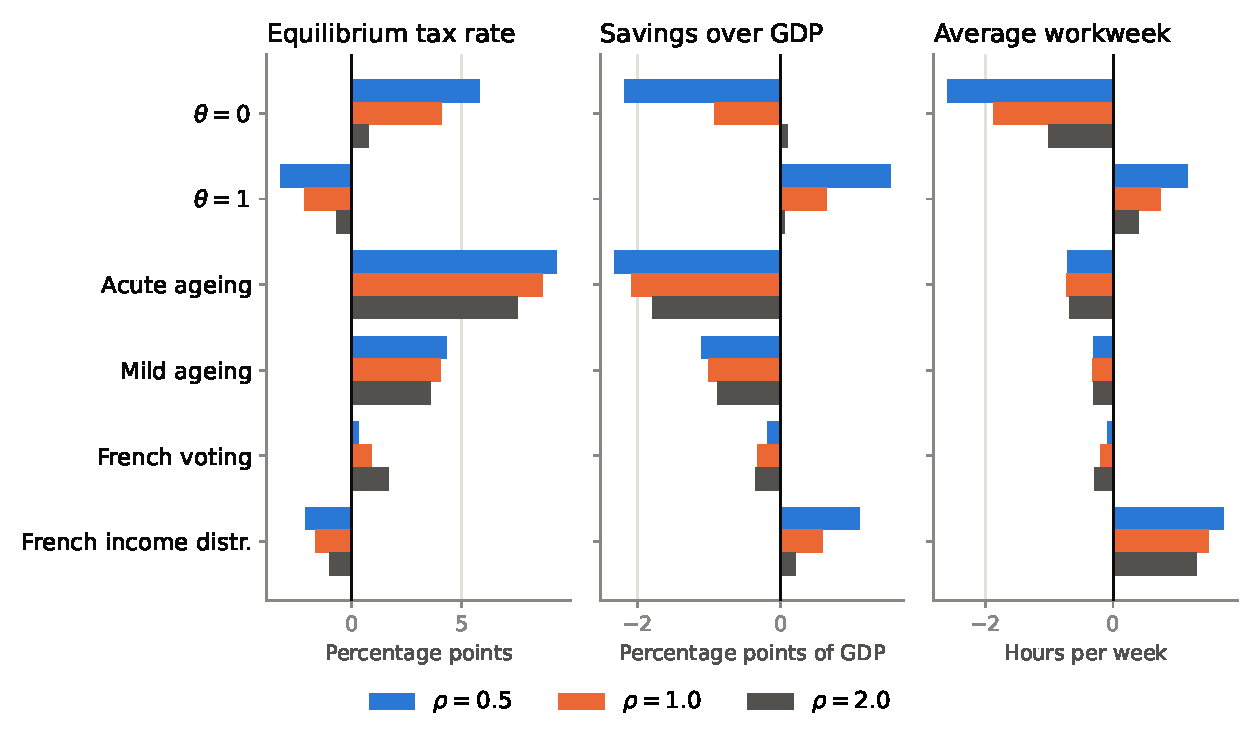
\includegraphics[width=\linewidth]{Figs/US_overview_vectorX.pdf}
\begin{tablenotes}[flushleft]\footnotesize
    \item[] \textit{Note:} As figure \ref{fig:US:overview}, under the vector-$X_i$ calibration; the baseline levels are the baseline row of table \ref{table:US:pensChars_vectorX}.
\end{tablenotes}
\end{threeparttable}
\end{figure}



